%! TeX root = ../../main.tex

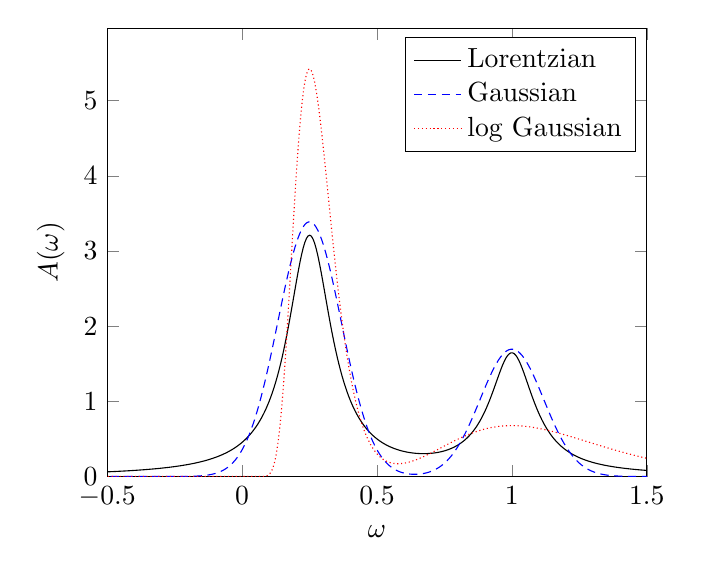
\begin{tikzpicture}
    \begin{axis}
        [
            xlabel=$\omega$,
            ylabel=$A(\omega)$,
            xmin=-0.5,
            xmax=1.5,
            ymin=0,
            legend cell align=left,
        ]

        % weight and locations of two poles
        \def\L{0.25}
        \def\W{1.0}
        \def\LL{1.0}
        \def\WW{0.5}

        % Lorentzian
        \def\DELTA{0.1}
        \addplot [color=black, domain=-1:2, samples=500] { \DELTA/pi*(\W/((x-\L)^2 + \DELTA^2) + \WW/((x-\LL)^2 + \DELTA^2))};
        \addlegendentry{Lorentzian}

        % Gaussian
        \def\SIGMA{0.11774100225154747} % HWHM sqrt(2*ln(2))*\DELTA
        \addplot [color=blue, densely dashed, domain=-1:2, samples=500] { 1/sqrt(2*pi*\SIGMA^2)*(\W*exp(-(x-\L)^2 / 2/ \SIGMA^2) + \WW*exp(-(x-\LL)^2 / 2 / \SIGMA^2))};
        \addlegendentry{Gaussian}

        % logarithmic Gaussian
        \def\B{0.4}
        \addplot [color=red, densely dotted, domain=-1:2, samples=900] { x > 0 ? exp(-\B^2 / 4) / (\B*sqrt(pi)) * (\W / \L *exp(-ln(x/\L)^2 / \B^2) + \WW / \LL *exp(-ln(x/\LL)^2 / \B^2)) : 0 };
        \addlegendentry{log Gaussian}
    \end{axis}
\end{tikzpicture}
